\documentclass{article}

\usepackage[utf8]{inputenc}
\usepackage[english]{babel}

\usepackage{amsmath,amsfonts,amssymb}
\usepackage{fullpage}
\usepackage{verbatim}
\usepackage{mathabx}

\usepackage{tikz,pgfplots}

\pgfplotsset{
  width=150mm,height=100mm,
  major grid style={thin,dotted,color=black!50},
  minor grid style={thin,dotted,color=black!50},
  grid,
  every axis/.append style={
    line width=0.5pt,
    tick style={
      line cap=round,
      thin,
      major tick length=4pt,
      minor tick length=2pt,
    },
  },
  legend cell align=left,
  legend pos=north west,
}

%%%%%%%%%%%%%%%%%%%%%%%%%%%%%%%%%%%%%%%%%%%%%%%%%%%%%%%%%%%%%%%%%%%%%%%%%%%%%%%%

\begin{document}

\title{LCE-Queries}
\author{Alexander Herlez}
%\maketitle



% IMPORT-DATA stats time-2019-06-26-14-51-59.txt

\begin{center}
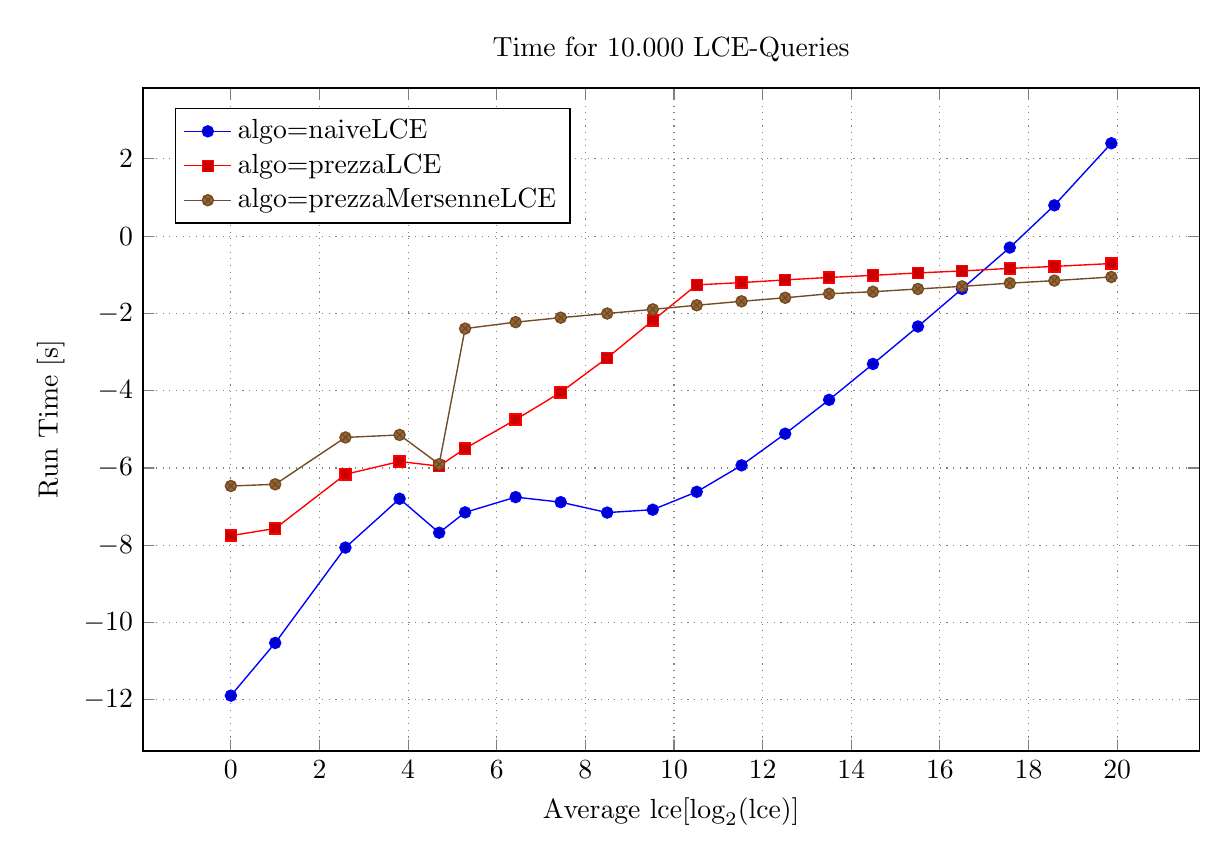
\begin{tikzpicture}
  \begin{axis}[
    title={Time for 10.000 LCE-Queries},
    xlabel={Average lce[$\log_2$(lce)]},
    ylabel={Run Time [s]},
    ]

    %% MULTIPLOT(algo) SELECT LOG(2, aveLCE) AS x, time AS y, MULTIPLOT
    %% FROM stats GROUP BY MULTIPLOT,x  ORDER BY MULTIPLOT,x
    \addplot coordinates { (0.0,-11.8928) (1.0,-10.5288) (2.58496,-8.06005) (3.80735,-6.7965) (4.70044,-7.67659) (5.2854,-7.14937) (6.42626,-6.75415) (7.44294,-6.88459) (8.49185,-7.15471) (9.51964,-7.08021) (10.5127,-6.61724) (11.5241,-5.93194) (12.5085,-5.11363) (13.4995,-4.23618) (14.4891,-3.30792) (15.505,-2.33805) (16.4986,-1.36436) (17.5768,-0.294406) (18.5825,0.798275) (19.8688,2.40501) };
    \addlegendentry{algo=naiveLCE};
    \addplot coordinates { (0.0,-7.75133) (1.0,-7.5655) (2.58496,-6.16452) (3.80735,-5.83215) (4.70044,-5.95223) (5.2854,-5.49394) (6.42626,-4.74863) (7.44294,-4.0427) (8.49185,-3.14965) (9.51964,-2.1849) (10.5127,-1.2599) (11.5241,-1.20177) (12.5085,-1.13184) (13.4995,-1.06844) (14.4891,-1.01392) (15.505,-0.950857) (16.4986,-0.900613) (17.5768,-0.834141) (18.5825,-0.783546) (19.8688,-0.707956) };
    \addlegendentry{algo=prezzaLCE};
    \addplot coordinates { (0.0,-6.46664) (1.0,-6.42254) (2.58496,-5.20945) (3.80735,-5.14423) (4.70044,-5.90254) (5.2854,-2.39151) (6.42626,-2.22552) (7.44294,-2.10938) (8.49185,-2.00154) (9.5216,-1.89427) (10.5127,-1.78821) (11.5241,-1.68573) (12.5085,-1.59469) (13.4995,-1.49075) (14.4891,-1.43832) (15.505,-1.3667) (16.4986,-1.29903) (17.5768,-1.21677) (18.5825,-1.15055) (19.8688,-1.05651) };
    \addlegendentry{algo=prezzaMersenneLCE};

  \end{axis}
\end{tikzpicture}
\end{center}

\end{document}
